% =====================================================================
% DIGEST -- the unrolled-Transformer (URformer) evaluation result.
% Short, scannable version of paper/spl2/haatim_structural_priors_evaluation.tex
%
% Single experiment family: the Track D URformer study.
%   trackD_urformer/            model, config, training
%   reports/trackD_stage2..5*   attribution, control, balanced loss, pilots
%   reports/trackD_pilot_three_way.json
% N=32, K=3, P=20 unless stated; SNR ~ U[-10,20] dB; RSR 10 dB; T=10 layers;
% 1,586,900 parameters; 80k training samples; 2000 paired test realisations.
% Every numeric claim carries a % SRC comment naming its store.
% =====================================================================
\documentclass[11pt]{article}

\usepackage[a4paper,margin=2.1cm,top=1.9cm,bottom=1.9cm]{geometry}
\usepackage{amsmath,amssymb}
\usepackage{graphicx}
\usepackage{booktabs}
\usepackage{enumitem}
\usepackage{xcolor}
\usepackage[hidelinks]{hyperref}
\usepackage[font=small,labelfont=bf,skip=4pt]{caption}
\usepackage{titlesec}
\usepackage{float}
% Keep text flowing around figures instead of leaving half-empty pages.
\renewcommand{\topfraction}{0.92}
\renewcommand{\bottomfraction}{0.75}
\renewcommand{\textfraction}{0.06}
\renewcommand{\floatpagefraction}{0.75}
\setcounter{topnumber}{3}
\setcounter{bottomnumber}{2}
\setcounter{totalnumber}{5}

\definecolor{ink}{HTML}{1a1a1a}
\definecolor{tag}{HTML}{6b6b6b}
\color{ink}

\titleformat{\section}{\large\bfseries}{\thesection.}{0.6em}{}
\titlespacing*{\section}{0pt}{14pt}{6pt}
\setlist[itemize]{leftmargin=1.1em,itemsep=2pt,topsep=3pt}
\setlist[enumerate]{leftmargin=1.4em,itemsep=3pt,topsep=3pt}
\setlength{\parskip}{4pt}
\setlength{\parindent}{0pt}

\newcommand{\bG}{\mathbf{G}}
\newcommand{\bS}{\mathbf{S}}
\newcommand{\bB}{\mathbf{B}}
\newcommand{\bW}{\mathbf{W}}
\newcommand{\bZ}{\mathbf{Z}}

\begin{document}

\begin{center}
{\LARGE\bfseries Do Structural Priors Actually Help}\\[3pt]
{\LARGE\bfseries Unrolled Channel Estimators?}\\[8pt]
{\large Results digest --- Rydberg atomic receivers}\\[6pt]
{\normalsize Abdullah Haatim \quad$\cdot$\quad Department of Electrical and
Electronics Engineering}\\
{\normalsize BITS Pilani --- Pilani Campus}
\end{center}

\vspace{2pt}
\hrule height 0.6pt
\vspace{10pt}

{\small
Short version of the unrolled-Transformer study. One experiment family
throughout: $N=32$, $K=3$, $P=20$ unless stated, SNR $\sim\mathcal{U}[-10,20]$
dB, $10$ unrolled layers, $1{,}586{,}900$ parameters, $80$k training samples,
$2000$ paired test realisations. Simulation only.
\par}

\vspace{6pt}

% =====================================================================
\section{The finding, in one paragraph}
% =====================================================================

We built an unrolled Transformer channel estimator (``URformer'') for the
magnitude-only Rydberg problem, added a Hankel low-rank structural prior inside
the loop, and measured a clear \textbf{$+1.209$~dB} advantage at high SNR. We
believed it. Then we ran a control to characterise where that advantage came
from --- and the control removed it. Under matched training the same contrast
is \textbf{$+0.078$~dB}, a fifteenfold collapse.

The reason is a training convention so common it is rarely stated. The loss is
a \emph{per-sample normalised} error averaged over a wide SNR range. Low-SNR
samples have far larger normalised error, so they dominate the average:
\textbf{$89.7\%$ of the gradient comes from trials below $5$~dB.} The high-SNR
regime is therefore underfitted, and \emph{any} mechanism that improves
high-SNR behaviour looks like it is adding information. A structural prior is
exactly such a mechanism.

\textbf{The first casualty of this control was our own method.} We report it
because a result that survives an author's attempt to keep it is worth more
than one that was never tested.

% =====================================================================
\section{Where the gain actually comes from}
% =====================================================================

Before the control, we decomposed the unrolled estimator's $+3.345$~dB
improvement over the classical EM-GS baseline.

\begin{itemize}
% SRC: reports/trackD_stage2_report.md, attribution at 80k
\item The learned per-layer \textbf{filter} ($980$ parameters) contributes
$0.147$~dB.
\item The \textbf{attention block} ($1{,}585{,}920$ parameters) contributes the
remaining $3.198$~dB --- \textbf{$96\%$ of the total}.
\item The filter's contribution \emph{falls} with more data
($0.193\to0.147$~dB from $20$k to $80$k samples), which is what a
never-capacity-limited $980$-parameter component should do.
% SRC: reports/trackD_stage3_report.md, X1 -> U1
\item \textbf{Unrolling itself does real work}, independently of attention.
Against a matched control that applies one Transformer block to a
\emph{converged} EM-GS estimate instead of unrolling, the unrolled estimator
gains $+0.920$~dB (CI $[+0.888,+0.988]$), winning on $86.5\%$ of trials.
\end{itemize}

So the architecture is doing something real. The question the rest of this
digest answers is whether the \emph{structural prior} added on top of it is.

\begin{figure}[!t]
\centering
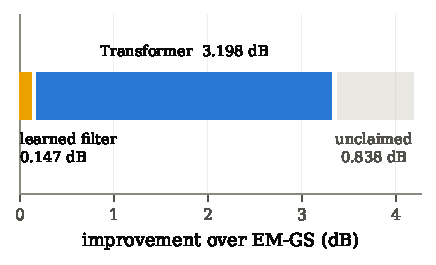
\includegraphics[width=0.50\textwidth]{fig/fig1_attribution.pdf}
\caption{\textbf{Attribution of the unrolled estimator's gain over EM-GS} at
$80$k training samples. The attention block accounts for $96\%$ of the
$+3.345$~dB. ``Unclaimed'' is the remainder of the genie-aided least-squares
headroom --- a \emph{reference}, not a bound: it presumes the true phase of the
noiseless field, which no receiver has.}
\end{figure}

% =====================================================================
\section{The confound}
% =====================================================================

The training loss is the per-sample normalised error
$\|\hat\bG-\bG\|_F^2/\|\bG\|_F^2$, averaged over a batch spanning the whole SNR
range. A low-SNR realisation has a normalised error orders of magnitude larger
than a high-SNR one, so the average is dominated by the low-SNR tail. Measured
directly on our own estimator:

\begin{itemize}
% SRC: reports/trackD_stage5_results.json, C1_snr_balanced_P20.unweighted_shares
\item $89.7\%$ of the gradient comes from trials below $5$~dB.
\item The per-bin gradient share spans a factor of $30$ across the range
($0.465$ in the lowest bin against $0.015$ in the highest).
\end{itemize}

The consequence: the high-SNR regime is systematically underfitted, so anything
that helps there gets credited with supplying information it did not supply.

% =====================================================================
\section{The control, and what it did to our method}
% =====================================================================

The protocol is cheap, and we recommend running it before any structural prior
is credited.

\begin{enumerate}
\item \textbf{Measure} the per-bin gradient share of the training loss. If it
is far from uniform, the regime receiving least gradient is underfitted.
\item \textbf{Retrain both arms} --- structured and unstructured --- with
training concentrated on the regime of interest, matching data budget,
schedule, seed and initialisation.
\item \textbf{Re-measure the contrast.} What survives is attributable to the
prior. What does not was compensating for training inadequacy.
\end{enumerate}

Applied to our own estimator over $[5,20]$~dB:

\begin{table}[H]
\centering
\small
\begin{tabular}{lcc}
\toprule
& \textbf{Mixed-SNR training} & \textbf{Matched focused training} \\
\midrule
% SRC: reports/trackD_stage4_report.md
Structural advantage, SNR $\ge5$ dB & $+1.209$ dB & $+0.078$ dB (CI $[0.050,0.112]$) \\
\midrule
\multicolumn{3}{l}{\emph{Absolute NMSE gain from focused training, SNR $\ge5$ dB:}} \\
Unstructured arm & \multicolumn{2}{c}{$+2.653$ dB} \\
Structured arm & \multicolumn{2}{c}{$+1.629$ dB} \\
\bottomrule
\end{tabular}
\caption{A fifteenfold collapse. The mechanism is in the bottom half: the
\emph{unstructured} network gains far more from adequate high-SNR training than
the structured one does. Given proper gradient in that regime it learns the
array geometry by itself, leaving the explicit projection almost nothing to
add.}
\end{table}

\begin{figure}[!t]
\centering
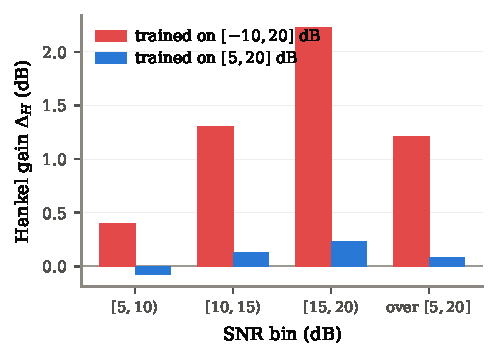
\includegraphics[width=0.50\textwidth]{fig/fig2_confound.pdf}
\caption{\textbf{The structural advantage before and after the control.} Both
arms are retrained identically; only the training SNR range differs. The
prior's apparent value was largely a proxy for the unstructured arm's
high-SNR underfitting.}
\end{figure}

\textbf{Scope of this negative result.} It holds at $N=32$, $K=3$, this data
budget and the pilot counts tested. It is \emph{not} a general claim that
structural priors cannot help unrolled estimators. Two counterweights from the
same study:

\begin{itemize}
\item The same prior applied to the \emph{classical} estimator --- where no
training adequacy is at stake --- gives a large and stable gain.
% SRC: reports/trackD_stage5_eval.json, C5_path_richness_ood, P10
\item Under a distribution shift in path richness, the structured network
degrades \emph{least} ($0.48$~dB against $0.73$~dB).
\end{itemize}

The prior buys robustness here. It is the in-distribution accuracy claim that
does not survive the control.

% =====================================================================
\section{The fix: rebalance the loss}
% =====================================================================

The confound is a property of the loss, so we fixed the loss. Each sample is
weighted by a static per-bin factor $w(b)=c/m(b)$, where $m(b)$ is the mean
per-sample normalised error in bin $b$, measured once before training and
scaled to unit mean weight. \textbf{No schedule, no tuning, no architectural
change} --- a few lines. It works as designed:

\begin{itemize}
% SRC: reports/trackD_stage5_results.json, C1_snr_balanced_P20.realized_shares
\item The per-bin gradient share now spans a factor of $1.9$, against $30$
before.
\item The share below $5$~dB falls from $0.897$ to $0.427$, against an ideal of
$0.5$ --- a slight over-correction.
\end{itemize}

And the estimation result is \textbf{better than we predicted}:

\begin{itemize}
% SRC: reports/trackD_stage5_eval.json, P13_balanced_vs_uniform_P20
\item Against an identically-trained unbalanced baseline, balancing gains
$+1.902$~dB at SNR $\ge5$~dB (CI $[+1.823,+1.986]$), rising monotonically to
$+2.628$~dB in the top bin.
\item We had \textbf{pre-registered a low-SNR cost} of $-0.10$ to $-0.40$~dB,
reasoning that the lowest bin's weight falls about eighteenfold. \textbf{There
was no cost}: the measured low-SNR change is $+0.135$~dB (CI
$[+0.101,+0.172]$). Those bins were over-served, not merely well-served.
\item The gap to the genie-aided reference at SNR $\ge5$~dB falls from
$+2.897$ to $+1.000$~dB.
\end{itemize}

\textbf{Rebalancing the loss recovers considerably more than the structural
prior appeared to offer} --- $+1.902$~dB against an apparent $+1.209$~dB --- at
a fraction of the complexity.

\begin{figure}[!t]
\centering
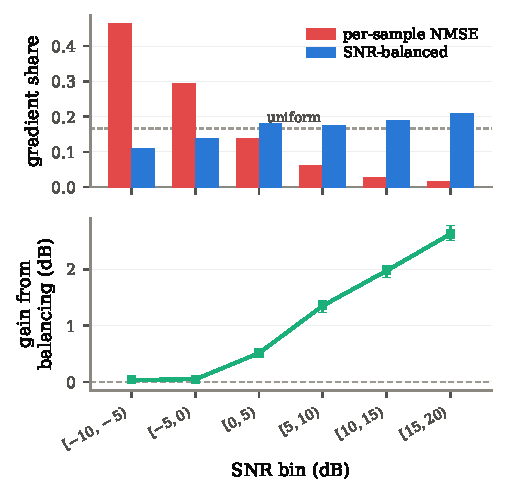
\includegraphics[width=0.50\textwidth]{fig/fig3_balanced_loss.pdf}
\caption{\textbf{Cause and effect.} \emph{Upper:} per-bin gradient share under
the per-sample normalised loss and under SNR balancing. \emph{Lower:} the
resulting per-bin gain, paired per-trial median with bootstrap $95\%$ CI. Below
$5$~dB the balanced estimator passes the genie-aided reference by up to
$1.99$~dB --- consistent rather than anomalous, since that reference is
restricted to unstructured least squares and an estimator that has learned the
channel geometry is not.}
\end{figure}

% =====================================================================
\section{A separate trap: pilot efficiency is not pilot-count generalization}
% =====================================================================

A pilot-count curve for a trained estimator can mean two different things, and
they are routinely reported as one: \textbf{generalization} (one model trained
at some $P_0$, evaluated at each $P$) or \textbf{efficiency} (a separate model
trained at each $P$). They are not close.

\begin{itemize}
% SRC: reports/trackD_stage5_eval.json, P14_P10 and P14_P35
\item Trained at $P=10$, the estimator beats the $P=20$ model evaluated there
by $+2.231$~dB pooled, with every bin's CI excluding zero.
\item At $P=35$ the corresponding margin is only $+0.635$~dB --- the model
generalizes \emph{upward} in pilot count far better than downward.
% SRC: reports/trackD_pilot_three_way.json
\item At $5$~dB the matched-trained estimator reaches $-7.52$~dB at $P=10$,
within $0.47$~dB of the genie-aided reference, while the $P=20$ model evaluated
there is $2.60$~dB short of it.
\item The clearest single symptom: the $P=20$ model is \textbf{worse at $P=25$}
($-11.13$~dB) \textbf{than at $P=20$} ($-11.27$~dB). More measurements, worse
estimate --- because the curve is tied to its training condition.
\end{itemize}

\begin{figure}[!t]
\centering
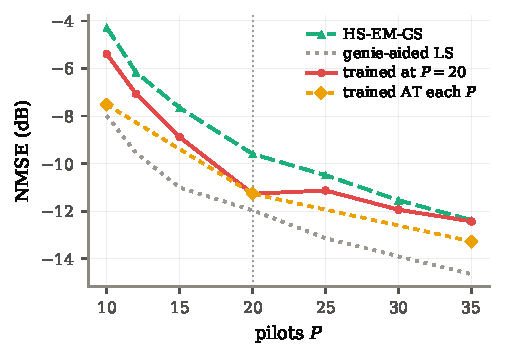
\includegraphics[width=0.50\textwidth]{fig/fig4_pilots_three_way.pdf}
\caption{\textbf{Pilot efficiency against pilot-count generalization} at
$5$~dB, on identical realisations. Dashed diamonds are separate networks
trained at each $P$; the solid curve is one network trained at $P=20$. Reported
as a single curve, these two quantities are indistinguishable to a reader ---
and they differ by $2.231$~dB.}
\end{figure}

% =====================================================================
\section{What this does and does not claim}
% =====================================================================

\begin{itemize}
\item \textbf{Not a critique of any specific paper.} The convention examined
here is near-universal, and our own estimator used it. Our earlier pilot curves
had the same ambiguity.
\item \textbf{Not a reproduction of prior work.} The URformer is implemented
faithfully on our geometric ULA model, but the operating point differs and
reaching the reported behaviour needed roughly four times the stated data
budget. Nothing here validates or refutes a published number.
\item \textbf{No bound is established.} The reference curve throughout is
genie-aided --- it presumes the true phase of the noiseless field --- and our
own balanced estimator passes it below $5$~dB.
\item \textbf{The negative result is scoped}, to $N=32$, $K=3$, one data budget
and the pilot counts tested. It is not a claim that structural priors cannot
help unrolled estimators anywhere.
\item \textbf{Simulation only.} No measured hardware, no recorded channel data.
\end{itemize}

% =====================================================================
\section{What to take away}
% =====================================================================

\begin{enumerate}
\item \textbf{Run the matched-adequacy control before crediting a structural
prior.} Measure the gradient share; retrain both arms on the regime of
interest; re-measure. It is cheap and it is decisive.
\item \textbf{Check the loss weighting before adding architecture.} A per-bin
reweighting of a few lines beat the structural prior it was competing with, at
no low-SNR cost.
\item \textbf{Say whether a pilot-count curve is efficiency or
generalization.} Here the two differ by $2.231$~dB.
\end{enumerate}

\vspace{10pt}
\hrule height 0.4pt
\vspace{6pt}

{\small\textcolor{tag}{Full version, with the attribution table, the
pre-registrations and the complete limitations:\\
\texttt{paper/spl2/haatim\_structural\_priors\_evaluation.pdf}. The companion
work on the classical estimator (HS-GS) is \texttt{paper/master/} and
\texttt{paper/summary/}. No experiment was rerun to produce this digest.}\par}

\end{document}
